\section{Experiments}

We assess the performance of the Base System on labyrinth environments. The robot is positioned in a starting location and it stochastically navigates the environment based on transition probabilities from states to states. We split the experiments into two cases. The first is the case of timing, where $\sum = \{\sigma\}$ and the second is with multiple observations. For timing, the goal is to make predictions about how long the agent will survive the environment. One can also ask conditional queries such as how long the agent should expect to survive given that t seconds have elapsed $f(\sigma^m|\sigma^n) = (eqns)$. For multiple observations we place the agent in the environment, let it transition between states for a fixed number of observations and then remove the agent. The goal for the multiple observation labyrinth will be to make predictions about seeing observation sequences. In both cases, we analyse the performance for M-PSRs of different model sizes with a fixed observation set. For each Base System M-PSR, we include all powers of 2 up to 256. For the heuristic based PSRs we learn 10 operators from the observations with the greedy learning algorithm for obtaining $\kappa$ described in (). To measure the performance of a PSR we use the following norm:
$||f - \hat{f}|| = \sqrt{\sum\nolimits_{x \in observations}(f(x) - \hat{f(x)})^2}$. We use this norm because of a bound presented by [AUTHORS], which states that (). The function f is obtainable explicitly for the environments which we consider as we have access to the underlying HMM of the environment. We compute approximations to this error norm, by fixing a set of strings T and summing over T. For the timing case, we take T to be the $\{sigma^k, k<=n\}$, while for the multiple observation case, we take all possible strings producible from the prefixes and suffixes in our dataset. That is, for the multiple observation case $T = \{p \cdot c, \forall p \in P, s \in S\}$.

\subsection{Learning PSRs for Timing}
For the timing case, we construct our empirical hankel matrix by including ${\sigma^i i<=n}$. With this choice, the empirical hankel matrix will be a nxn matrix with the prefixes and suffixes being the same.The parameter n depends on the application. For Double Loop environments we set n to be 300, while for pacMan it was 600. The important property that needs to be satisfied when choosing the parameter n is that enough observations are captured to learn a good model. Something here: $\lim_{ \to 2} f(x) = 5$ .

\subsection{Learning PSRs for Multiple Observations}

For multiple observations a slightly more complex approach is required to construct the empirical hankel matrix. For prefixes, we select the k most frequent prefixes from our observations set. For suffixes we take all suffixes that occur from our set of prefixes. This heuristic was given in previous work by [] and it showed that ().

\subsection{Double Loop Timing}

For timing, we start by considering a double loop environment. The lengths of the loops correspond to the number of states in the loop. Every time the agent transitions to a new state, a $sigma$ observation is produced.  An observation of $\sigma^{100}$ corresponds to the agent surviving the environment for 100 time units. The agent starts at the intersection of the two loops. At the intersection, the agent has a 50 percent chance of entering either loop. At intermediate states in the loops it simply moves to the next state in the loop with probability p and remains in its current state with probability 1-p. Exit states are located halfway between each loop. At an exit state, the agent has a 50 percent probability of exiting the environment. In figure 1, we learn a PSRs with 10000 observation sequences. We generate 10 PSRs and average their performance. 

\begin{figure}[ht!]
\centering
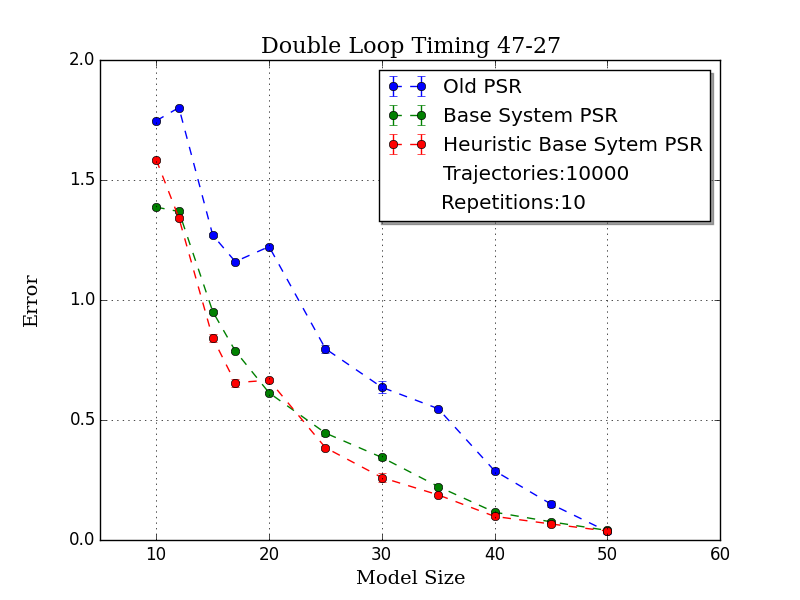
\includegraphics[width=60mm]{uCOREPICS/DoubleLoopTimingHeuristics47-27.png}
\caption{Double Loop Environment\label{overflow}}
\end{figure}

\begin{figure}[ht!]
\centering
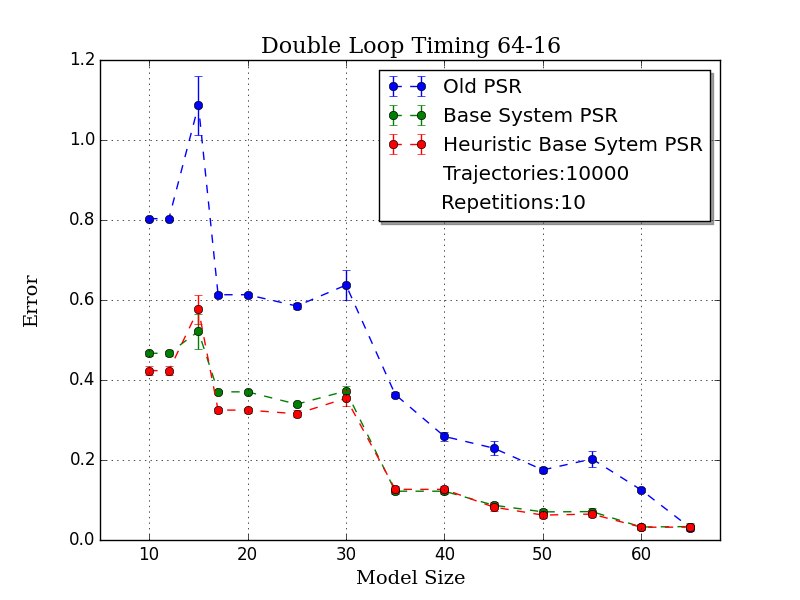
\includegraphics[width=60mm]{uCOREPICS/DoubleLoop64-16Heuristics.png}
\caption{Double Loop Environment\label{overflow}}
\end{figure}

\subsection{Pacman Timing}

We proceed to work with timing in a Pacman environment. The transition structure of this environment is shown in Figure 2. Edge weights vary from 1 to 3 and are stretched by a parameter which we call the stretch factor. Again we use 10000 observation sequences per PSR and compute the average error of 10 PSRs.

\begin{figure}[ht!]
\centering
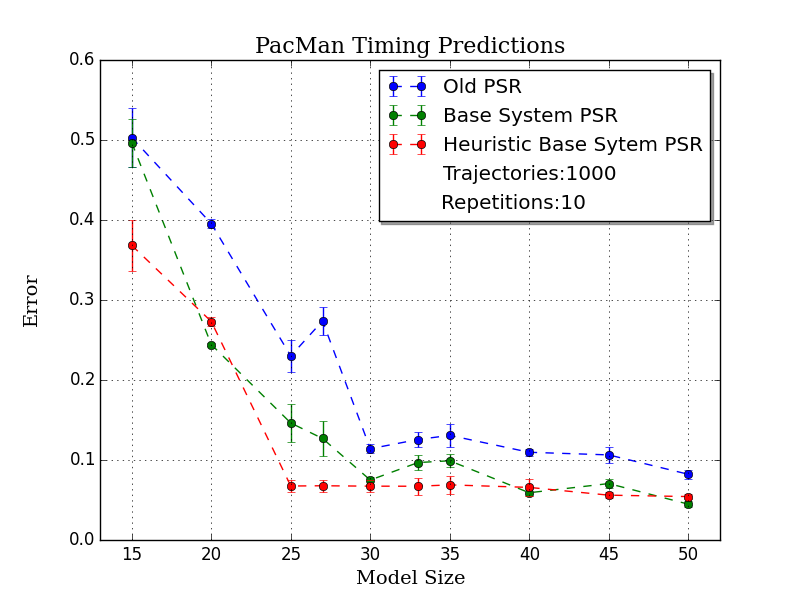
\includegraphics[width=60mm]{uCOREPICS/PacManTimingHeuristicsIncluded.png}
\caption{Double Loop Environment\label{overflow}}
\end{figure}

\subsection{Timing - Results}
As is demonstrated in figure 3, learning longer transitions provides a significant improvement over the standard for truncated models. The heuristic based approach performs slightly better than the powers of two method. For the double loop case the heuristic approach learns multiples of the loop lengths which results in partitions which use fewer operators. For Pacman, the operators that are learned are various multiples of the stretch factor, which once again shows that the greedy heuristic is effective. 

\subsection{Multiple Observations}

To test whether the Base System would translate to multiple observations we construct a double loop environment where one loop is green and the other is blue. The lengths of each loop are also varied. We fix the length of observations to be $loop1 + loop2 * 3$. To build empirical estimates of probabilities we set f(x)=prefix-occ(x)/num-strings-length>=x.

\subsection{Multiple Observations Results}

\begin{figure}[ht!]
\centering
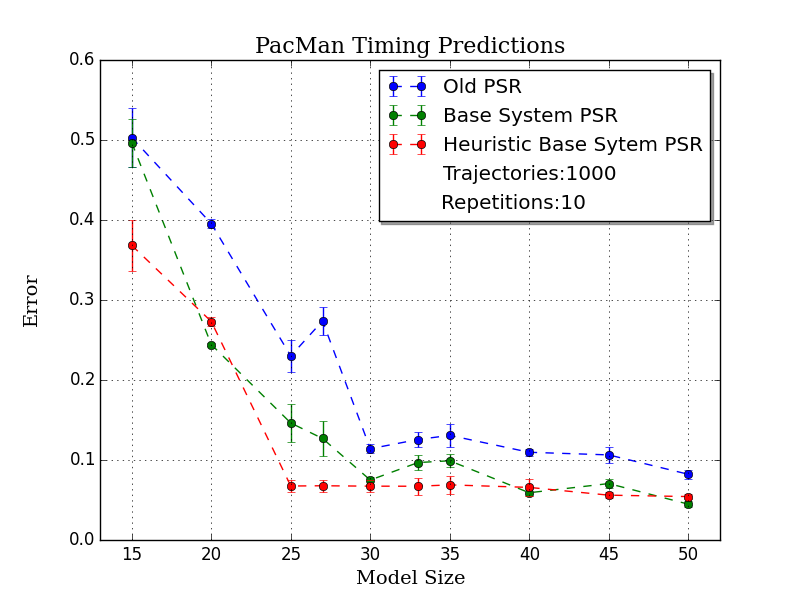
\includegraphics[width=60mm]{uCOREPICS/PacManTimingHeuristicsIncluded.png}
\caption{Double Loop Environment\label{overflow}}
\end{figure}
